\documentclass[12pt, final]{dalcsthesis}
\usepackage{graphicx}
\usepackage{subcaption}
\usepackage{amsmath}
\usepackage{algorithm}
\usepackage[noend]{algpseudocode}
\usepackage{hyperref}

\graphicspath{{../assets/experiments/aggregate_results/figures}{../assets/experiments/baseline/figures}}

\begin{document}
\bcshon
\title{Reinforcement Linear Genetic Programming}
\author{Urmzd Mukhammadnaim}
\defenceday{12}
\defencemonth{April}
\defenceyear{2023}
\convocation{May}{2023}

\supervisor{M. Heywood}
\reader{D. Arnold}
\reader{}

\nolistoftables
\nolistoffigures

\frontmatter

\nocite{*}

\begin{abstract}
	% Write a brief summary of the research, its purpose, and findings.
\end{abstract}

\begin{acknowledgements}
	I'd like to dedicate this piece of work to all those who've pushed me to continue my
	pursuit of education. My brother Frebarz, who always encouraged me to push a little further. My Mother, Khalima and my sister Rita, whom without in my life, I would've never started in the first place. I'd also like to thank Dr. Malcolm Heywood for
	his patience and support during the entirety of this thesis from conception to completion, and the opportunity to experience the world of academia.
\end{acknowledgements}

\mainmatter

\chapter{Introduction}
The rapid growth of technology and the increasing complexity of real-world problems demand efficient and effective optimization techniques. Evolutionary algorithms (EAs) have demonstrated significant potential in addressing these challenges by emulating the process of natural selection to search for optimal solutions. Linear Genetic Programming (LGP), a branch of Genetic Programming (GP), is one such EA that has gained attention in the field of computer science for its unique approach to tackling complex problems. By representing programs as a sequence of linear instructions, similar to what is found when programming imperatively, LGP allows for solutions that are not only interpretable but also more efficient to execute and manipulate.

However, one problem that arises in LGP is that programs within the framework require humans to explicitly configure the action-register pairings. A pairing consists of a register and an associated action that the framework executes upon a program's execution. With the use of these explicit action-register pairs, we reduce the exploration capabilities of the programs, leading to suboptimal solutions. To address this issue, we propose a novel approach that combines the power of LGP with the Q-Learning algorithm, a popular model-free reinforcement learning technique.

The resulting algorithm, Reinforced Linear Genetic Programming (RLGP), is then able to learn the optimal register-action assignments, potentially leading to more efficient and effective solutions. RLGP inherits the benefits of LGP, such as its linear representation and ease of manipulation while augmenting it with the adaptive capabilities of Q-Learning. This integration allows RLGP to explore and exploit the solution space more effectively, resulting in improved performance when addressing complex optimization problems.

We evaluate the performance of RLGP on a variety of benchmark problems, including the CartPole and MountainCar environments from the OpenAI Gym library \cite{1606.01540}. These environments provide challenging tasks that require sophisticated decision-making and control strategies, making them suitable for assessing the effectiveness of RLGP. We compare the baseline LGP framework with the augmented RLGP framework in terms of solution quality, convergence speed, and adaptability to dynamic problem domains.

By combining the strengths of LGP and Q-Learning, RLGP might represents a significant advancement in the field of evolutionary computation. This research not only contributes to the understanding of hybrid evolutionary algorithms but also paves the way for future work on incorporating reinforcement learning techniques into other EAs.

\chapter{Background}
\section{Linear Genetic Programming}
Linear Genetic Programming (LGP) is an advanced form of Genetic Programming (GP), a powerful machine learning technique introduced by Brameier and Banzhaf in their seminal work \cite{brameier2001comparison}. Unlike the traditional tree-based GP, LGP represents programs as a linear sequence of instructions, similar to assembly language or machine code. This representation offers several advantages, such as improved evolvability, efficient execution, and simplicity of crossover and mutation operations.

In LGP, programs are composed of registers and instructions, where each instruction manipulates the contents of registers using arithmetic, logical, or conditional operations. The fitness of a program is determined by its ability to solve a given problem, such as regression, classification, or optimization tasks. The evolutionary process is similar to that of canonical GP, but involves variation operators that act directly upon a linear set of instructions.

In their paper, Brameier and Banzhaf compared the performance of LGP to that of traditional GP and neural networks. They discovered that LGP had classification and generalization capabilities that were comparable to those of neural networks \cite{brameier2001comparison}. This finding was significant, as it demonstrated that LGP could serve as an alternative to neural networks for solving complex machine learning problems. Moreover, LGP's linear representation allows for more interpretable solutions, which is an important consideration in many applications where understanding the underlying model is crucial.

The paper further explored the benefits of LGP's linear representation, such as improved evolvability and more efficient execution. These advantages make LGP an attractive choice for solving complex problems, as it can produce high-quality solutions more quickly than traditional GP methods. Additionally, the simplicity of crossover and mutation operations in LGP ensures that the evolutionary process remains efficient and effective, allowing for the exploration of a diverse range of solutions.

Brameier and Banzhaf's work on LGP laid the foundation for further research into the capabilities and applications of this powerful machine learning technique. The findings of their paper highlight the potential of LGP as a robust and versatile machine learning approach, particularly in scenarios where both high performance and interpretability are required.

\section{Reinforced Genetic Programming}
In the RGP paper, Downing applied the Reinforced Genetic Programming approach to several benchmark problems, including function optimization and control tasks \cite{downing1995reinforced}. The results showed that RGP significantly outperformed traditional Genetic Programming and other baseline algorithms in terms of convergence speed, solution quality, and robustness. This demonstrated the effectiveness of incorporating Q-Learning into the genetic programming framework to guide the exploration and exploitation of the search space.

One of the key findings of the paper was that the combination of Genetic Programming and Q-Learning allowed RGP to adapt more efficiently to changing environments and problem landscapes. By utilizing the reinforcement signals from the environment, RGP could dynamically adjust its search strategy, making it more responsive to the changes in the problem domain. This ability to adapt and learn from the environment is particularly relevant to real-world problems, where the solution space may be dynamic, noisy, or uncertain.

The paper also introduced several novel techniques for integrating Q-Learning into the Genetic Programming framework, such as the use of Q-values to bias the selection of genetic operations and the incorporation of reinforcement signals into the fitness function. These innovations allowed RGP to leverage the strengths of both Genetic Programming and Q-Learning, resulting in a more powerful and flexible optimization algorithm.

In the context of Reinforced Linear Genetic Programming (RLGP), the findings of Downing's paper suggest that integrating Q-Learning into the LGP framework could yield similar benefits. By combining the global search capabilities of LGP with the local search and adaptation of Q-Learning, the resulting algorithm, which could be referred to as RLGP, may be able to tackle complex and dynamic problem domains more effectively.

\chapter{Methodology}
\section{Framework Overview}
We use the Rust programming language to implement the framework for our research. The framework is designed to be extensible and versatile, allowing
for various types of problems to be solved using LGP and RLGP. The framework is also designed to be easily configurable, allowing for extensive experimentation. The framework consists of several engines, which together implement the core functionality. The primary engines can categorized into one of several categories. Variation engines, which allow operations such as two point crossover and mutation, which consists of replacing the contents of an instruction. Stochastic engines, which allow for random states and programs to be generated. Evaluation engines such as the which allows the system to determine the fitness of a program. With this in mind, we describe our representation of a program and the algorithms implemented by these engines to train the programs.

\subsection{Program Representation}
A program can be thought of a container holding instructions and a set of registers. A single instruction consists of the source register index, the target register index and the operation to be performed as well as a mode flag. The mode flag is used to determine where the target register is located. If set, the mode flag indicates that the target register is located outside the program. In other words, the value held in the target register is given by an external source (such as the features of some dataset or the environmment state). We can represent the program as a sequence of instructions in the following format: $R[x] <op>= R[y]$ where R represents the registers, $x$ and $y$ represent the source and target register indices respectively, and $<op>$ represents the operation to be performed. In our case, we only allow four operations; addition (+),
subtraction (-), multiplication(*) and division (/) by 2. Division is done by a non-zero constant as to prevent divsion by zero errors that would likely crash the system. This representation makes it easy to implement variation operations, but also easy to digest for humans unlike other machine learning techniques and tree-based programs, which convolute the internal process used to solve a problem.

\subsection{The Algorithm}

We outline the main algorithm below, as well as the operations that enable
the algorithm to function. The algorithm is implemented in the Core, which is responsible for the main loop of the algorithm. The core algorithm involves initializing a population of programs, evaluating the programs against the desired task using the FitnessEngine and associated learning type, ranking the individuals based on their fitness score,
dropping the least fit individuals, as specified by GAP, then producing a new population by applying filling the
dropped spots by children produced by the remaining individuals in the population.

\begin{algorithm}[hb]
	\caption{Genetic Algorithm}
	\begin{algorithmic}[1]
		\Procedure{GeneticAlgorithm}{}
		\State $P \gets \Call{InitializePopulation}{n\_individuals}$
		\For{$i \in \{0, 1, \dots, n\_generations - 1\}$}
		\State $\Call{Evaluate}{P_{i}, N\_TRIALS}$
		\State $\Call{Rank}{P_{i}}$ \Comment{Rank individuals directly by fitness}
		\State $P_{i+1} \gets \Call{Clone}{P}$
		\State $P_{i+1} \gets \Call{Survive}{P_{i+1}, GAP}$ \Comment{Drop GAP\% of the least fit individuals}
		\State $parents \gets \Call{Select}{P_{i+1}}$
		\State $P_{i+1} \gets \Call{Variation}{P_{i+1}}$
		\EndFor
		\State \Return $P_{n\_generations}$
		\EndProcedure
	\end{algorithmic}
\end{algorithm}

\begin{algorithm}[hb]
	\caption{Breed: Two-Point Crossover}
	\label{alg:breed}
	\begin{algorithmic}[1]
		\Procedure{Breed}{$P_1, P_2$}
		\Comment{Given two programs, $P_1$ and $P_2$}
		\State{$P_1', P_2' \gets \Call{Clone}{P_1, P_2}$}
		\Comment{Clone the programs to prevent accidental mutation}
		\State{$I_1 \gets P_1'.instructions$}
		\State{$I_2 \gets P_2'.instructions$}
		\Comment{Get instructions from both parents}
		\State{$p_1, p_2 \gets \Call{RandomChunk}{I_1, I_2}$}
		\Comment{Randomly select a chunk of the instructions from each clone}
		\State{$I_1[p_1:p_2], I_2[p_1:p_2] \gets I_2[p_1:p_2], I_1[p_1:p_2]$}
		\Comment{Swap the chunks}
		\State \textbf{return} $P_1', P_2'$
		\Comment{Return the clones}
		\EndProcedure
	\end{algorithmic}
\end{algorithm}

\begin{algorithm}[hb]
	\caption{Mutate}
	\label{alg:mutate}
	\begin{algorithmic}[1]
		\Procedure{Mutate}{$P$}
		\Comment{Given a program}
		\State{$I \gets \Call{RandomInstruction}{P.instructions}$}
		\Comment{Randomly select an instruction}
		\State{$I' \gets \Call{GenerateRandomInstruction}{}$}
		\Comment{Generate a new instruction}
		\For{$prop \in \{operation,source, target\}$}
		\State{$r \gets \Call{RandomNumber}{0, 1}$}
		\If{$r < 0.5$}
		\State{\Call{Replace}{$I, I', prop$}}
		\Comment{Replace the property with a new value with a probability of 0.5}
		\EndIf
		\EndFor
		\Comment{For each property of the instruction}
		\State{$P.instructions \gets \Call{ReplaceInstruction}{P.instructions, I, I'}$}
		\Comment{When replacing target, also replace mode to ensure valid programs}
		\State \textbf{return} $P$
		\Comment{Return the child}
		\EndProcedure
	\end{algorithmic}
\end{algorithm}

\begin{algorithm}[hb]
	\caption{Generate}
	\label{alg:generate}
	\begin{algorithmic}[1]
		\Procedure{Generate}{$N, max\_instructions$}
		\State{$n \gets \Call{Random}{1, max\_instructions}$}
		\Comment{Generate a random number of instructions}
		\State{$R \gets \Call{GenerateRegisterSet}{N + 1}$}
		\Comment{Create a register set with N+1 registers}
		\State{$I \gets \Call{GenerateInstructions}{n}$}
		\Comment{Generate instructions}
		\State{$P \gets \Call{CreateProgram}{R, I}$}
		\Comment{Create a program by encapsulating the registers with the instructions}
		\State \textbf{return} $P$
		\Comment{Return the program}
		\EndProcedure
	\end{algorithmic}
\end{algorithm}

\begin{algorithm}[hb]
	\caption{Fitness}
	\label{alg:fitness-baseline}
	\begin{algorithmic}[1]
		\Procedure{Fitness}{$P, inputs, expected\_outputs$}
		\Comment{Given a program}
		\State{$score \gets 0$}
		\For{$i \in inputs$}
		\State{$output \gets \Call{Execute}{P, i}$}
		\Comment{Execute the program for each input}
		\State{$action \gets \Call{Argmax}{output.action\_registers}$}
		\Comment{Argmax over the action registers}
		\If{$action = expected\_outputs[i]$}
		\State{$score \gets score + 1$}
		\Comment{Increment the fitness if the argmax matches the expected output}
		\EndIf
		\EndFor
		\State{$accuracy \gets \frac{score}{|inputs|}$}
		\Comment{Divide the total score by the number of inputs}
		\State \textbf{return} $accuracy$
		\Comment{Return accuracy (fitness)}
		\EndProcedure
	\end{algorithmic}
\end{algorithm}

\section{Sanity Testing}
As a means of ensuring that the framework was implemented correctly, we developed four tests.
The first test (Figure \ref{fig:iris_baseline}) is a baseline test that only uses clones. As demonstrated,
all individuals converge to the best fitness score given enough generations. The second test (Figure \ref{fig:iris_mutation})
ensures that mutation is working correctly. As demonstrated, the fitness score increases over time. The third test (Figure \ref{fig:iris_crossover})
does the same, but for the two point crossover (breed) operation. The final test (Figure \ref{fig:iris_full}) ensures that both
are able to work together.

\begin{figure}
	\centering
	\begin{subfigure}[b]{0.48\textwidth}
		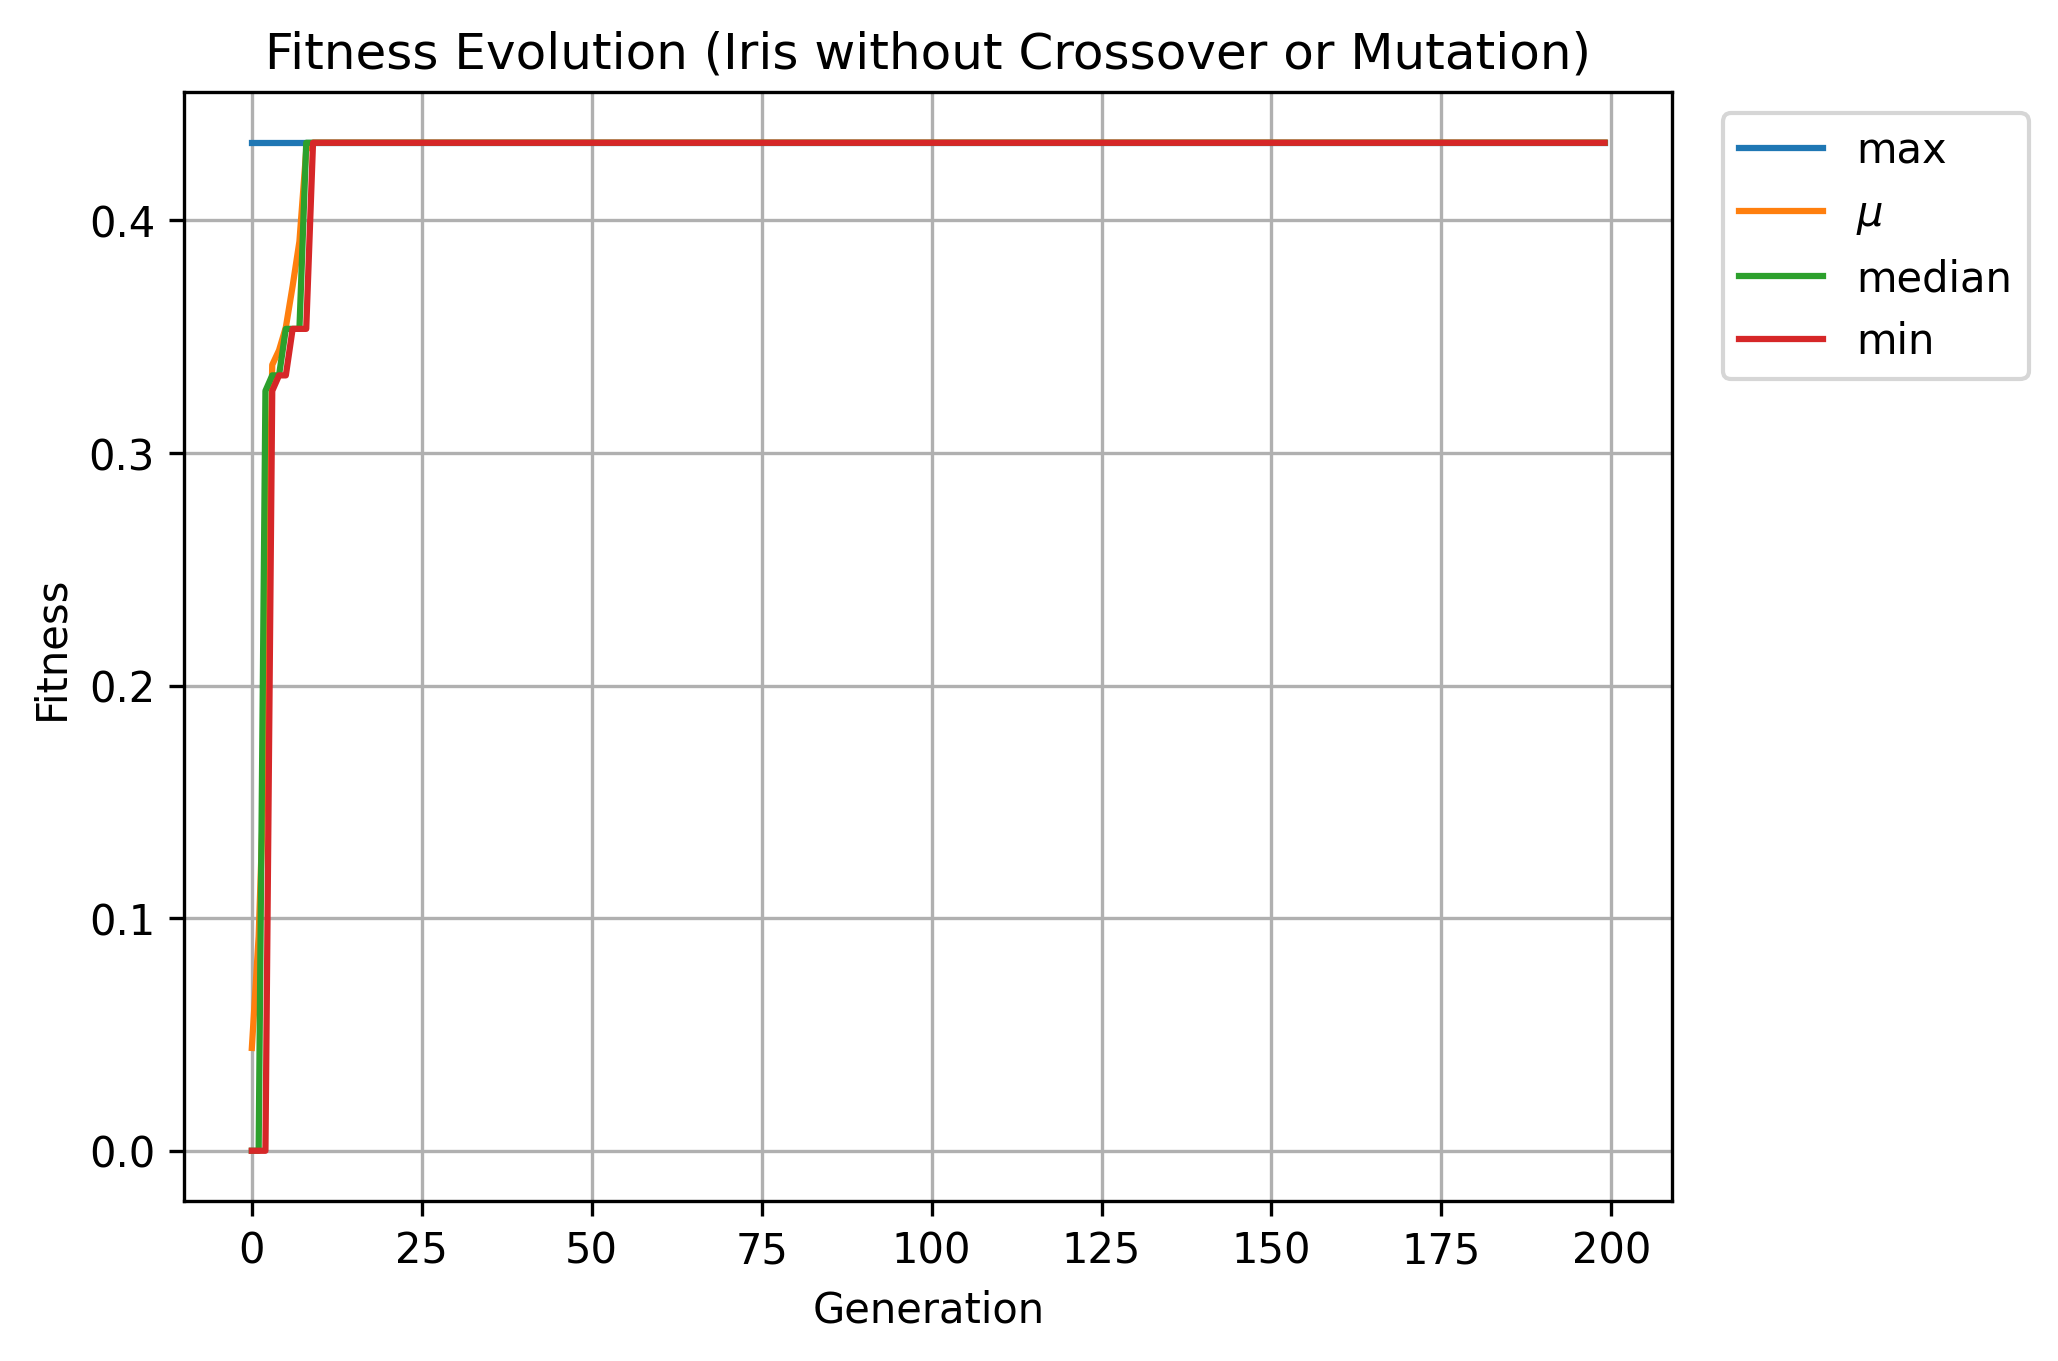
\includegraphics[width=\textwidth]{iris_baseline.png}
		\caption{LGP Without Variation On Iris}
		\label{fig:iris_baseline}
	\end{subfigure}
	\hfill
	\begin{subfigure}[b]{0.48\textwidth}
		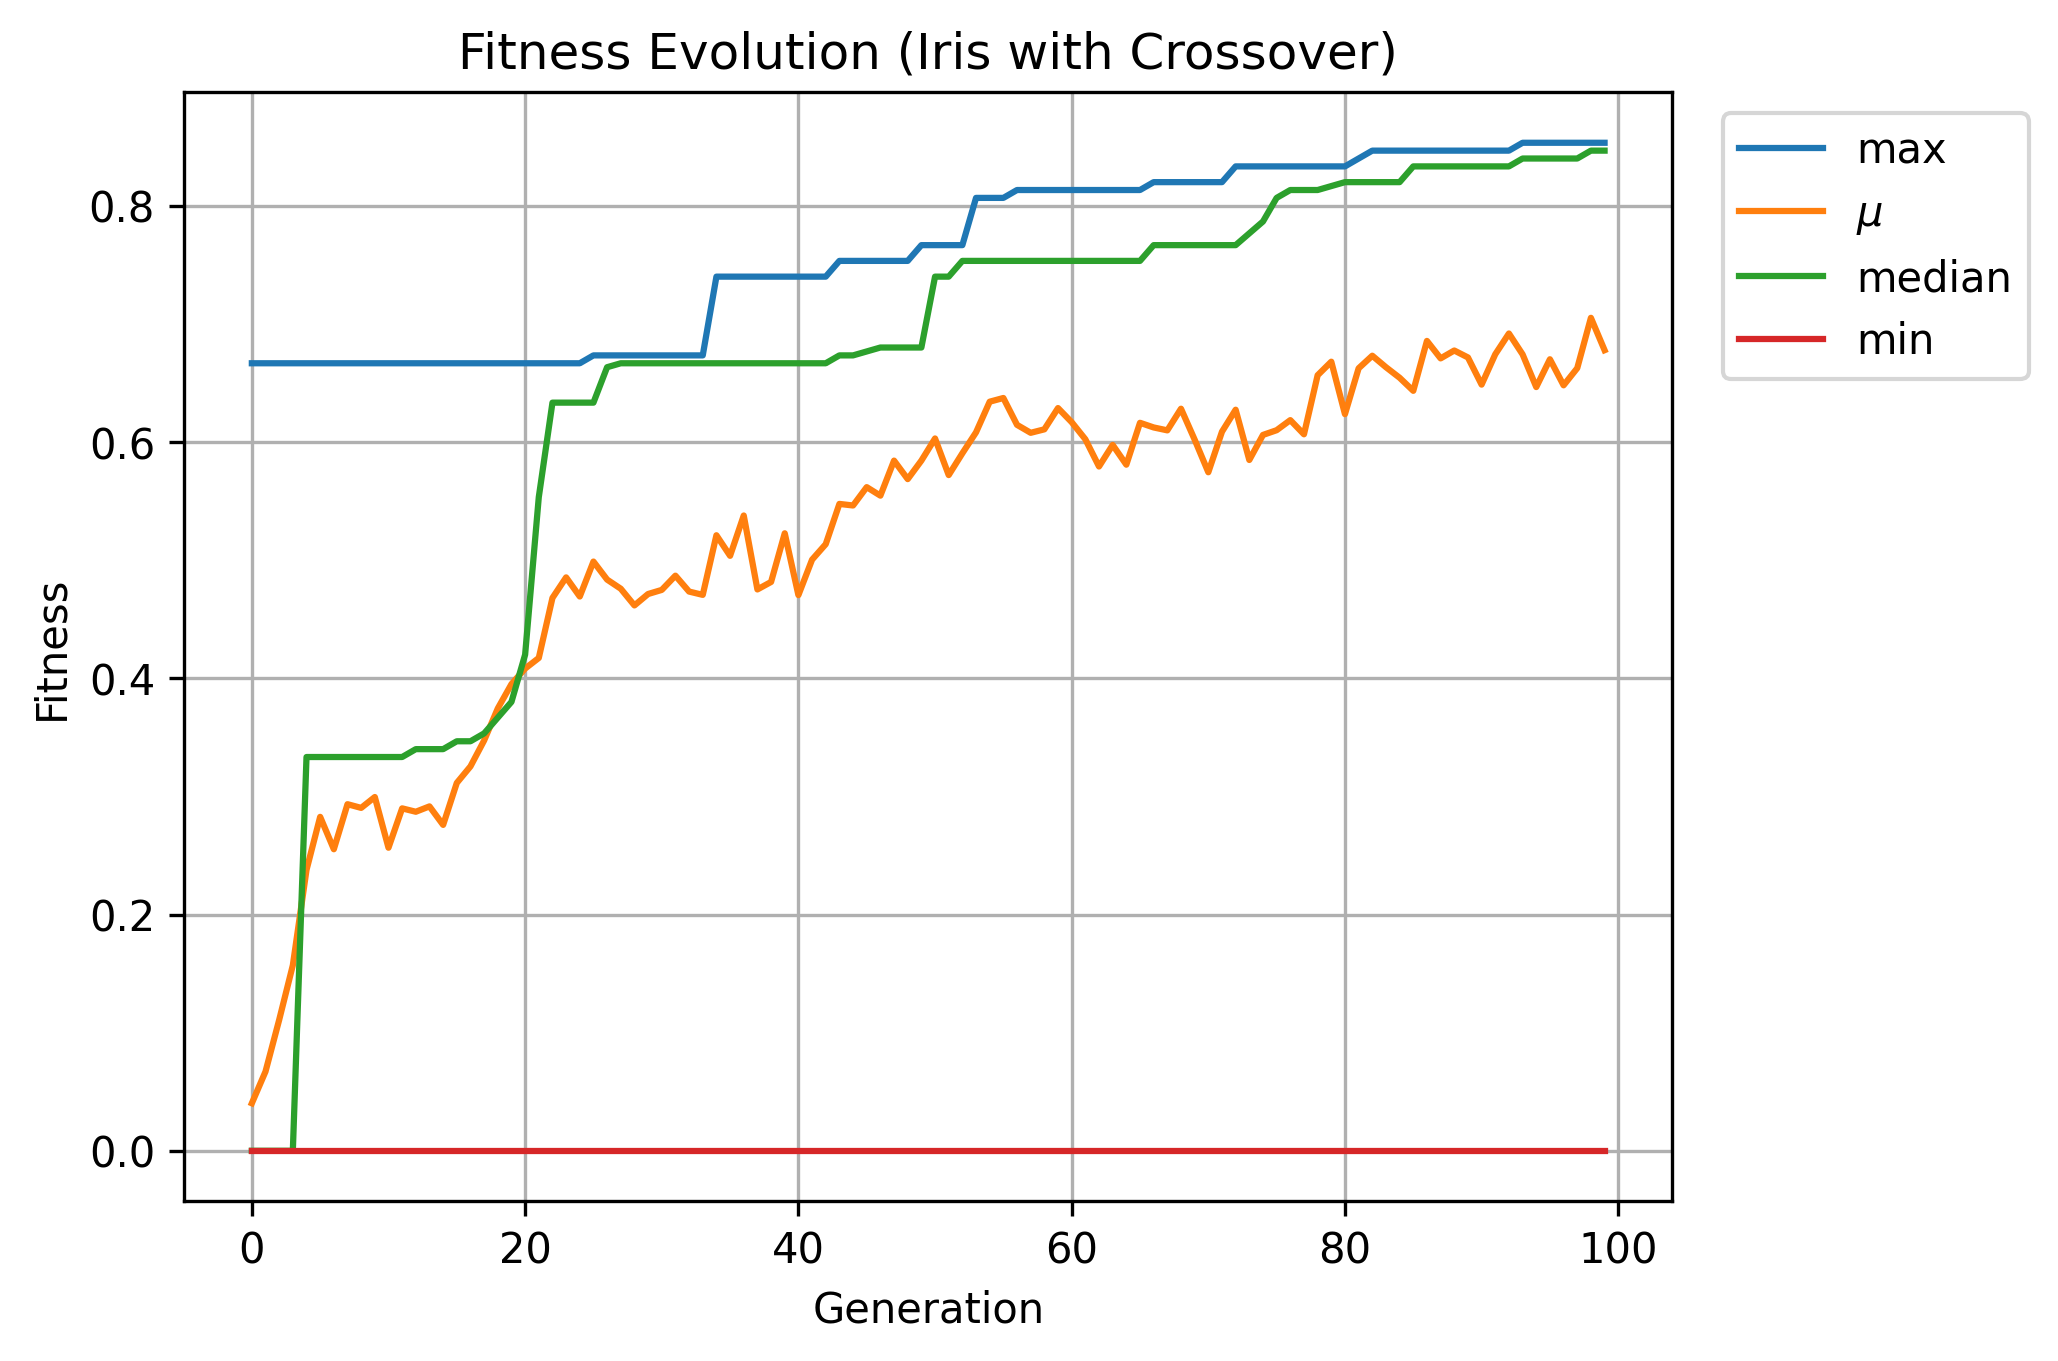
\includegraphics[width=\textwidth]{iris_crossover.png}
		\caption{LGP With Breed On Iris}
		\label{fig:iris_crossover}
	\end{subfigure}

	\medskip

	\begin{subfigure}[b]{0.48\textwidth}
		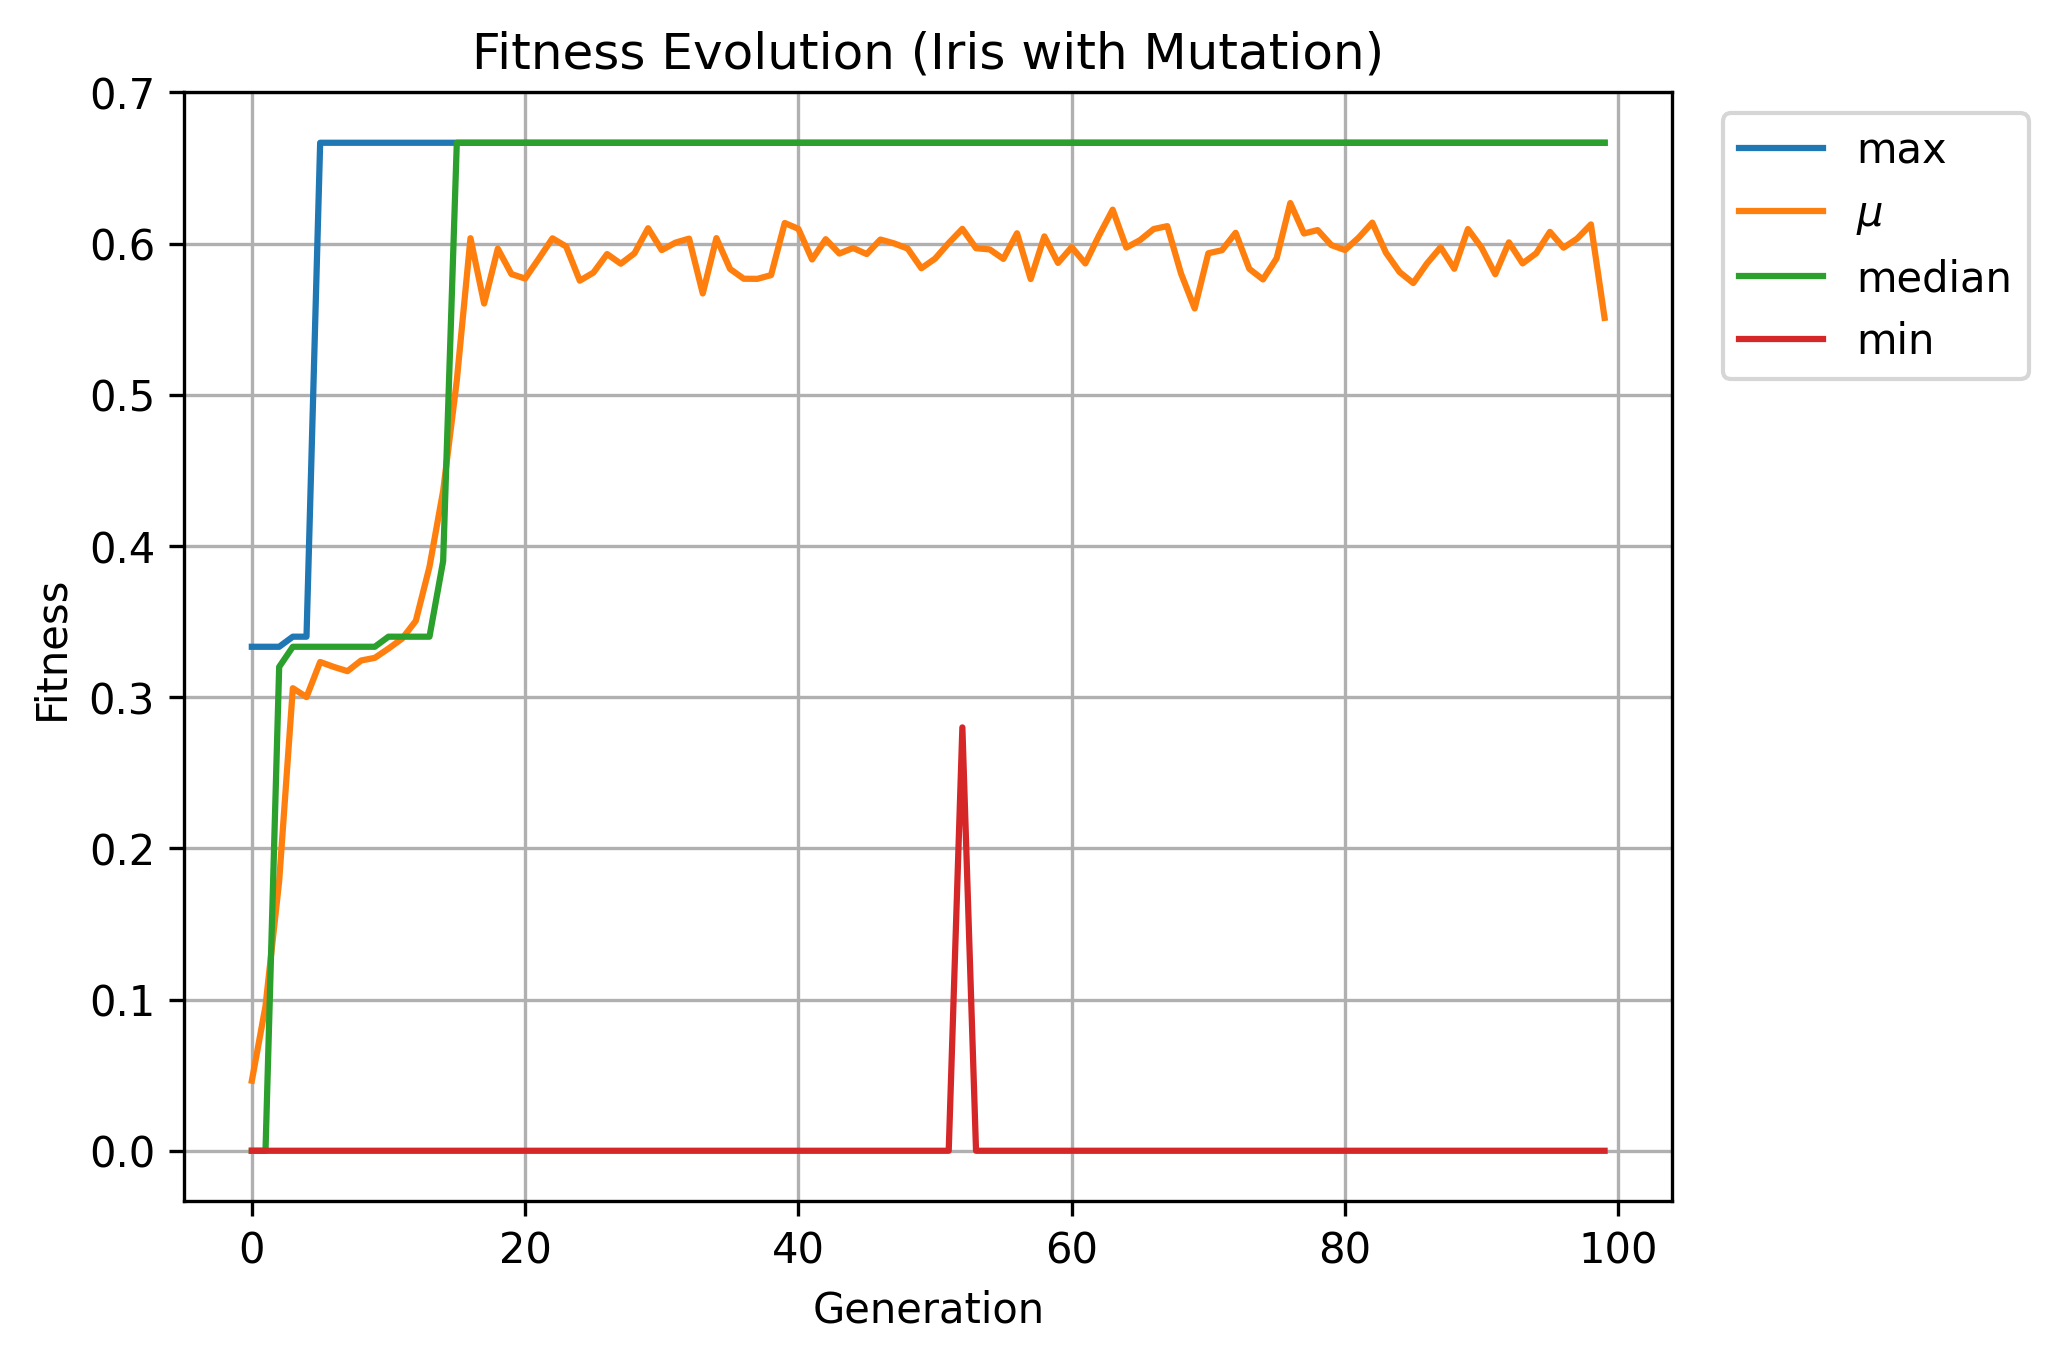
\includegraphics[width=\textwidth]{iris_mutation.png}
		\caption{LGP Using Only Mutation On Iris}
		\label{fig:iris_mutation}
	\end{subfigure}
	\hfill
	\begin{subfigure}[b]{0.48\textwidth}
		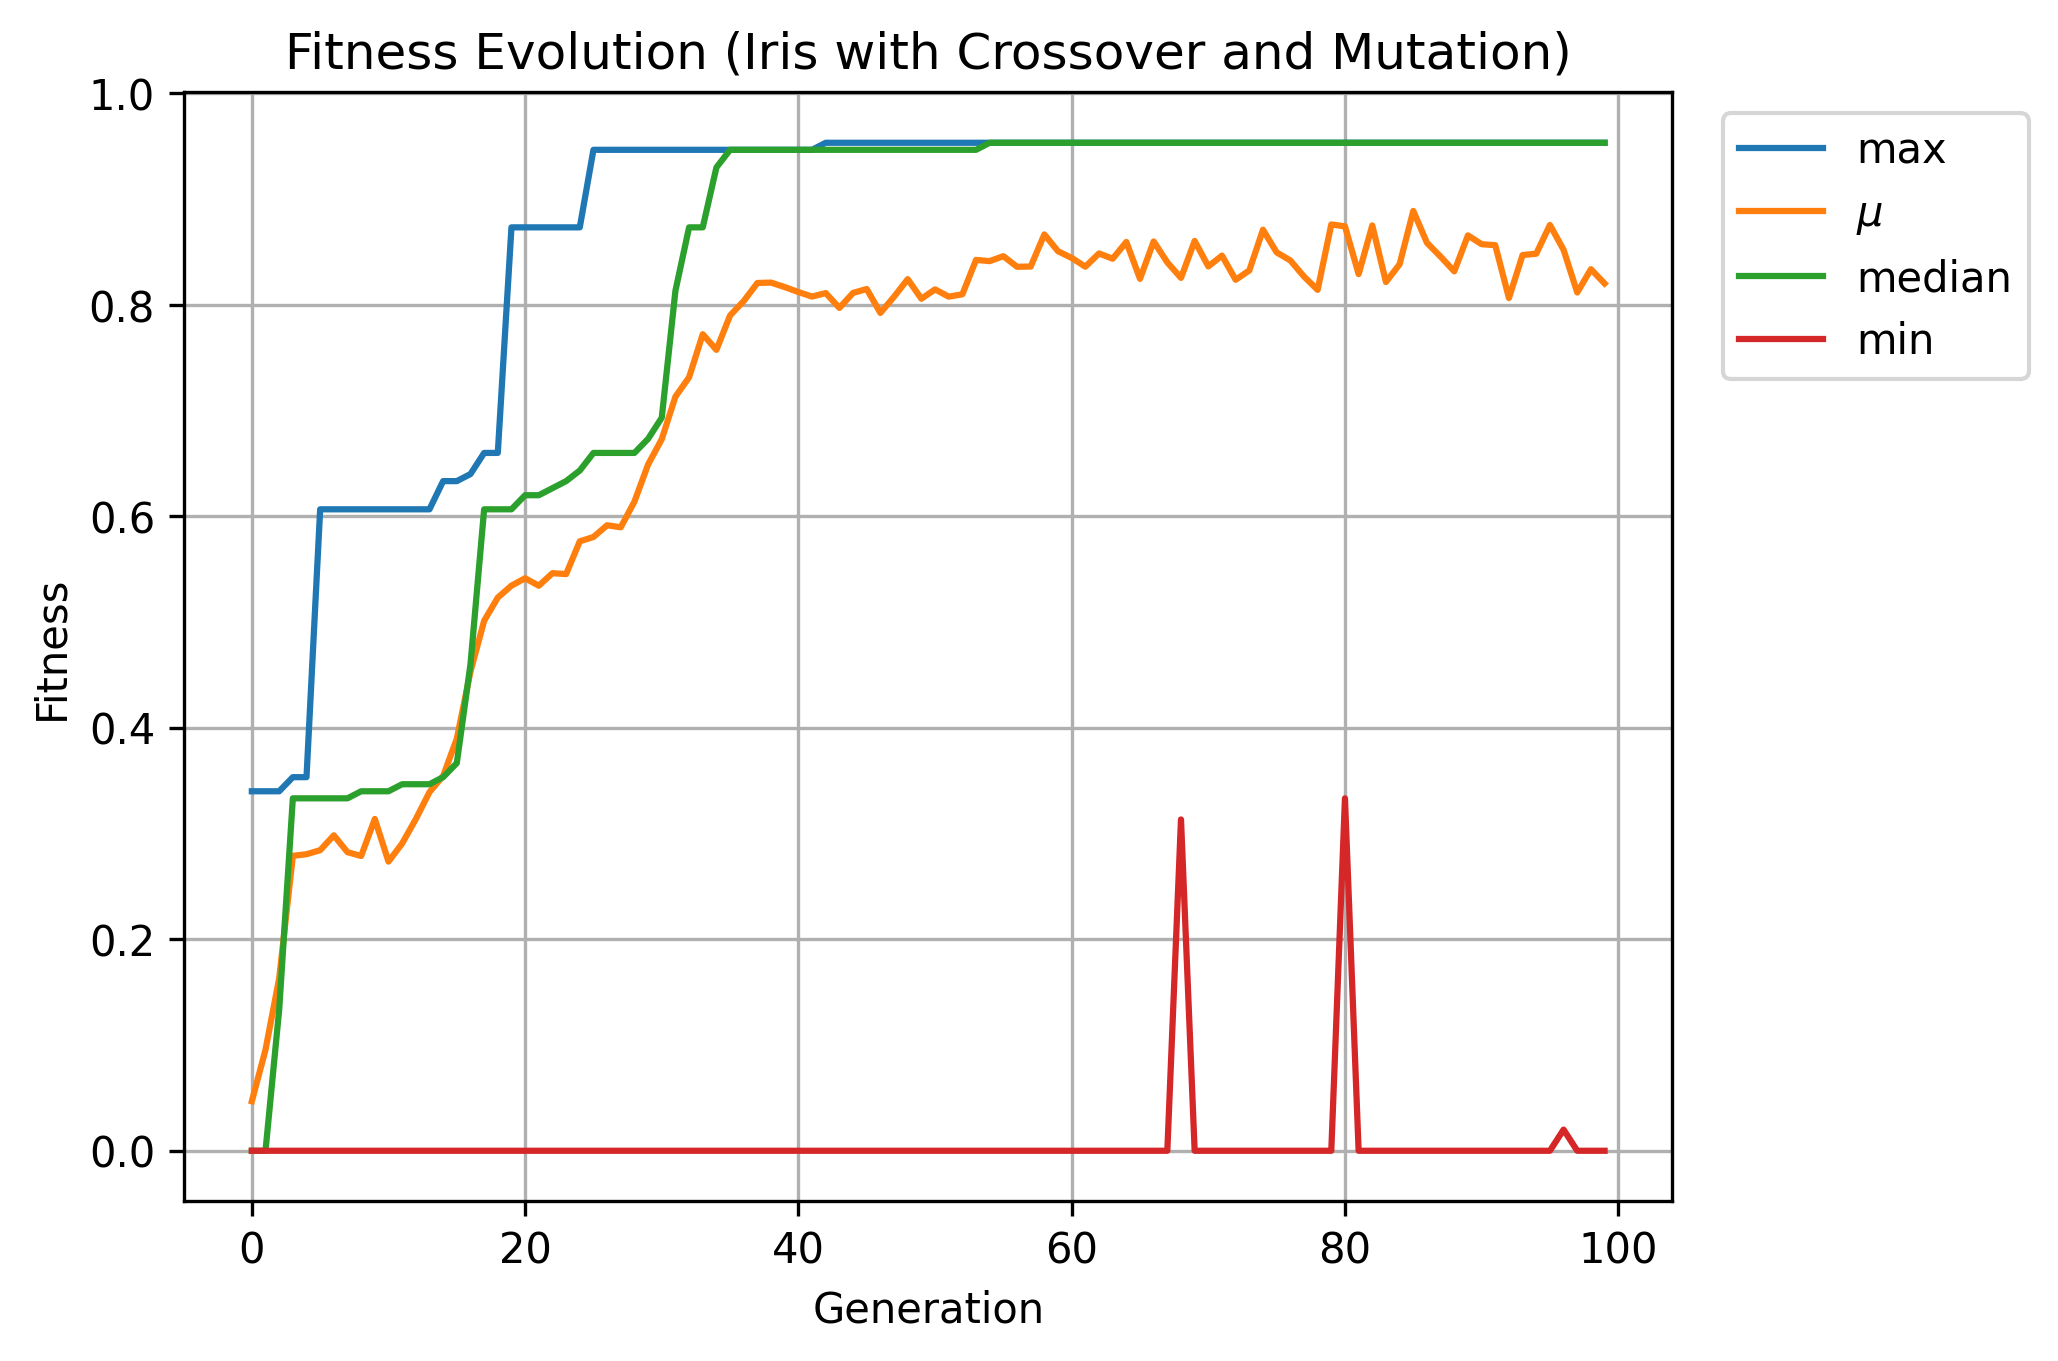
\includegraphics[width=\textwidth]{iris_full.png}
		\caption{LGP Using Both Mutation and Breeding On Iris}
		\label{fig:iris_full}
	\end{subfigure}

	\caption{Performance comparison of different genetic programming methods on iris dataset}
	\label{fig:iris_comparison}
\end{figure}

\section{Reinforcement Learning Integration}
We extend the fitness algorithm to work with both a Rust port of the OpenAI mountain car environment (mountain-car-v0) \cite{1606.01540} and the OpenAI cartpole environment (cartpole-v1) \cite{1606.01540}.

For the mountain-car-v0 environment, the agent's goal is to drive a car up a steep hill. The car is subject to gravity and has limited power. The car must learn to rock back and forth to build momentum before reaching the goal area at the top of the hill. The environment has two state variables representing the position, and velocity of the car. The car has three possible actions: push left, push right, or no push. The reward function for the environment gives a value of $-1$ at each time step until the car reaches the goal area, at which point the reward becomes $0$. The problem is considered solved when the car reaches the goal area with an average reward of -110 over 100 consecutive trials.

For the cartpole-v1 environment, the agent's goal is to balance a pole on top of a cart that can move left or right. The pole is subject to gravity, and the goal is to keep the pole upright for as long as possible. The environment has four continuous state variables representing the position and velocity of the cart and pole. The cart has two possible actions: move left or move right. The reward function for the environment gives a value of $1$ at each time step that the pole remains upright. The problem is considered solved when the pole remains upright for at least $195$ consecutive time steps over 100 consecutive trials.

With this in mind, we outline an alternative fitness algorithm used to baseline the framework on classical reinforcement learning problems, Algorithm \ref{alg:fitness-rl}.

\begin{algorithm}[hb]
	\caption{Fitness}
	\label{alg:fitness-rl}
	\begin{algorithmic}[1]
		\Procedure{Fitness}{$P, env$}
		\Comment{Given a program and an environment}
		\State{$score \gets 0$}
		\For{$i \in N_EPISODES$}
		\State{$done \gets False$}
		\While{$done = False$}
		\State{$output \gets \Call{Execute}{P, observation}$}
		\Comment{Execute the program for each input}
		\State{$action \gets \Call{Argmax}{output.action\_registers}$}
		\Comment{Argmax over the action registers}
		\State{$observation, reward, done, info \gets env.step(action)$}
		\Comment{Step the environment}
		\State{$score \gets score + reward$}
		\EndWhile
		\EndFor
		\State \textbf{return} $score$
		\EndProcedure
	\end{algorithmic}
\end{algorithm}


\section{Q Learning Integration}
We extend Algorithm \ref{alg:fitness-rl} further to support Q Learning (Algorithm \ref{alg:fitness-rlq}).
The Q Table consists of a 2D array of size $N_R \times N_A$, where $N_R$ is the number of registers the program can work with and $N_A$ is the number of available actions an agent can take. The Q Table is initialized to all zeros and updates only a different register has been selected. The Q Table is updated using the following formula.
\begin{equation}
	Q(R[x_t], a_t) \leftarrow Q(R[x_t], a_t) + \alpha \left(r_{t+1} + \gamma \max_a Q(R[x_{t+1}], a) - Q(R[x_t], a_t)\right)
\end{equation}

In this formula, $Q$ represents the Q Table, $R$ represents the set of registers, $a$ represents the available actions, $r_{t+1}$ is the reward at time step $t+1$, $\alpha$ is the learning rate, and $\gamma$ is the discount factor. The value $x_t$ represents the current state, while $x_{t+1}$ represents the next state. The update rule calculates the new Q value for the current state-action pair based on the observed reward and the maximum Q value for the next state.

\begin{algorithm}[hb]
	\caption{Q Learning LGP Fitness}
	\label{alg:fitness-rlq}
	\begin{algorithmic}[1]
		\Function{EvalFitness}{$P, S$}
		\State $sc \gets 0$
		\State $cur\_as \gets \Call{GetActionState}{S, P}$
		\If{$cur\_as = \text{None}$}
		\State \Return $-\infty$
		\EndIf
		\While{$st \gets \Call{S.Get}{} \neq \text{None}$}
		\State $rw \gets \Call{st.ExecuteAction}{cur\_as.action}$
		\State $sc \gets sc + rw$
		\If{$\Call{st.IsTerminal}{}$}
		\State \textbf{break}
		\EndIf
		\State $next\_as \gets \Call{GetActionState}{st, P}$
		\If{$next\_as = \text{None}$}
		\State \Return $-\infty$
		\EndIf
		\If{$cur\_as.register \neq next\_as.register$}
		\State $\Call{P.q\_table.Update}{cur\_as, rw, next\_as}$
		\EndIf
		\State $cur\_as \gets next\_as$
		\EndWhile
		\State \Return $sc$
		\EndFunction
	\end{algorithmic}
\end{algorithm}

\section{Experimental Setup}

In this section, we outline the experimental setup used to evaluate the performance of the proposed Q-Learning LGP algorithm in comparison to the baseline LGP. The experiments were conducted in two main stages: hyperparameter optimization and performance evaluation.

\subsection{Hyperparameter Optimization}

First, we utilized the Optuna hyperparameter optimization library \cite{akiba2019optuna} to find the optimal parameters for the baseline LGP programs. Optuna is a flexible and efficient hyperparameter optimization framework that allows for the automatic exploration of hyperparameter spaces in search of the best settings for a given algorithm.

Once the optimal parameters for the baseline LGP programs were identified, we conducted a separate search using Optuna to find the optimal Q-Learning constants for the Reinforced Linear Genetic Programming (RLGP) programs. This process aimed to fine-tune the RLGP algorithm's performance by selecting the most suitable Q-Learning parameters based on the problem domain and the characteristics of the LGP framework.

\subsection{Performance Evaluation}

After obtaining the optimal parameters for both baseline LGP and RLGP, we proceeded with the performance evaluation phase. This stage involved conducting 100 experiments, each consisting of 100 trials. The goal of these experiments was to assess the effectiveness and robustness of the RLGP algorithm compared to the baseline LGP across multiple runs and problem instances.

For each experiment, we calculated the mean, median, minimum, and maximum performance scores obtained by both baseline LGP and RLGP. These summary statistics provided a comprehensive overview of the algorithms' performance, highlighting their strengths and weaknesses across different trials and problem instances.

Finally, we plotted the average results (mean, median, min, max) for each experiment to visually compare the performance of the baseline LGP and RLGP algorithms. This visualization allowed us to identify trends and patterns in the algorithms' performance and gain insights into the benefits of incorporating Q-Learning into the LGP framework.

By following this experimental setup, we aimed to provide a thorough and unbiased evaluation of the proposed Q-Learning LGP algorithm, demonstrating its potential advantages over the baseline LGP and paving the way for future research and development in this area.

\chapter{Analysis}

This chapter analyzes the performance of a population of programs trained using Linear Genetic Programming (LGP)
and a population of programs trained using Linear Genetic Programming Reinforced with Q-Learning (LGP-Q). The programs
are trained on the cartpole-v1 and mountain-car-v0 environments \cite{1606.01540} as mentioned in the previous chapter.
Once the results are explained, we analyze them to provide insight into the impact of Q-Learning on the performance of LGP. Note that we use the definition of done as referenced in the leaderboards, see \href{https://github.com/openai/gym/wiki/Leaderboard}{OpenAI Gym Leaderboard Wiki}. This means that terms such for results as maximum, mean, median and min are the statistics for experiments averaged over 100 trials.

\section{Experimental Results}

\subsection{Cart Pole}

Figure \ref{fig:cart-pole-comparison} shows a comparison of the two programs' performance. The baseline program achieved a maximum score of 150, while the LGP-Q program achieved a maximum score of 120. The median score for the baseline program was 150, with an average score of 115. The LGP-Q program had a median score of 120, with an average score of 106.

The LGP-Q program was able to converge faster to a score of 120 than the baseline LGP program. However, once it reached 120, it began to plateau at around 15 generations. In contrast, the LGP program converged slower and reached a higher score before plateauing around 80 generations. These observations were consistent across the maximum, median, and mean fitness scores.

Overall, while neither program was able to solve the cartpole-v1 environment, the LGP-Q program showed a faster convergence to a reasonable score, albeit with a lower maximum score than the baseline LGP program.

\begin{figure}[hb]
	\centering
	\begin{subfigure}{1.0\textwidth}
		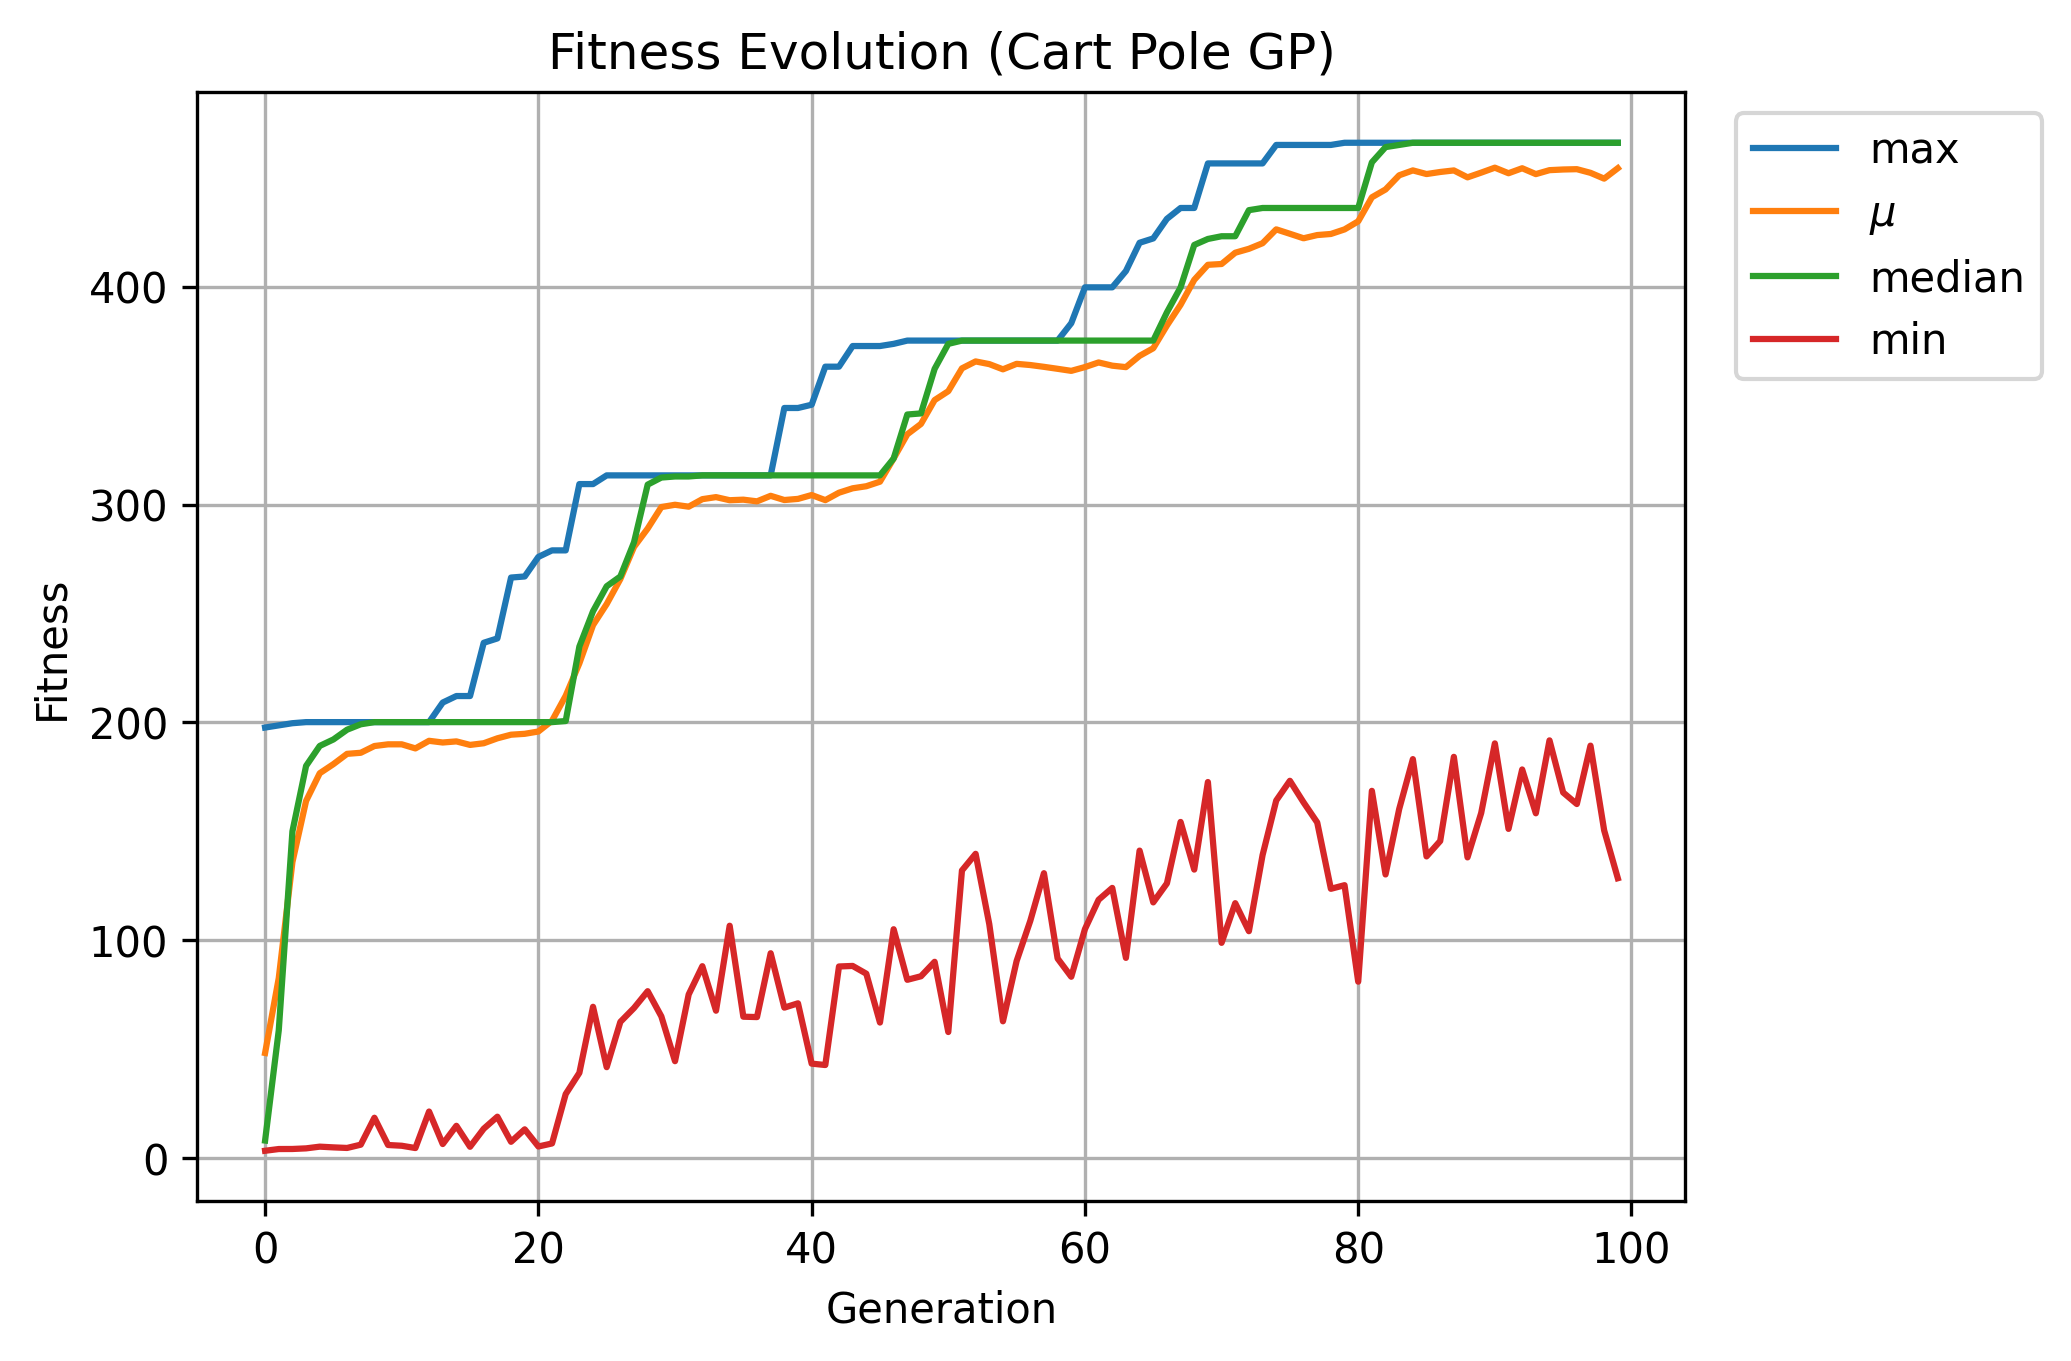
\includegraphics[width=\linewidth]{cart_pole_lgp.png}
		\caption{Baseline Linear Genetic Programming}
		\label{fig:cart-pole-lgp}
	\end{subfigure}
	\hfill
	\begin{subfigure}{1.0\textwidth}
		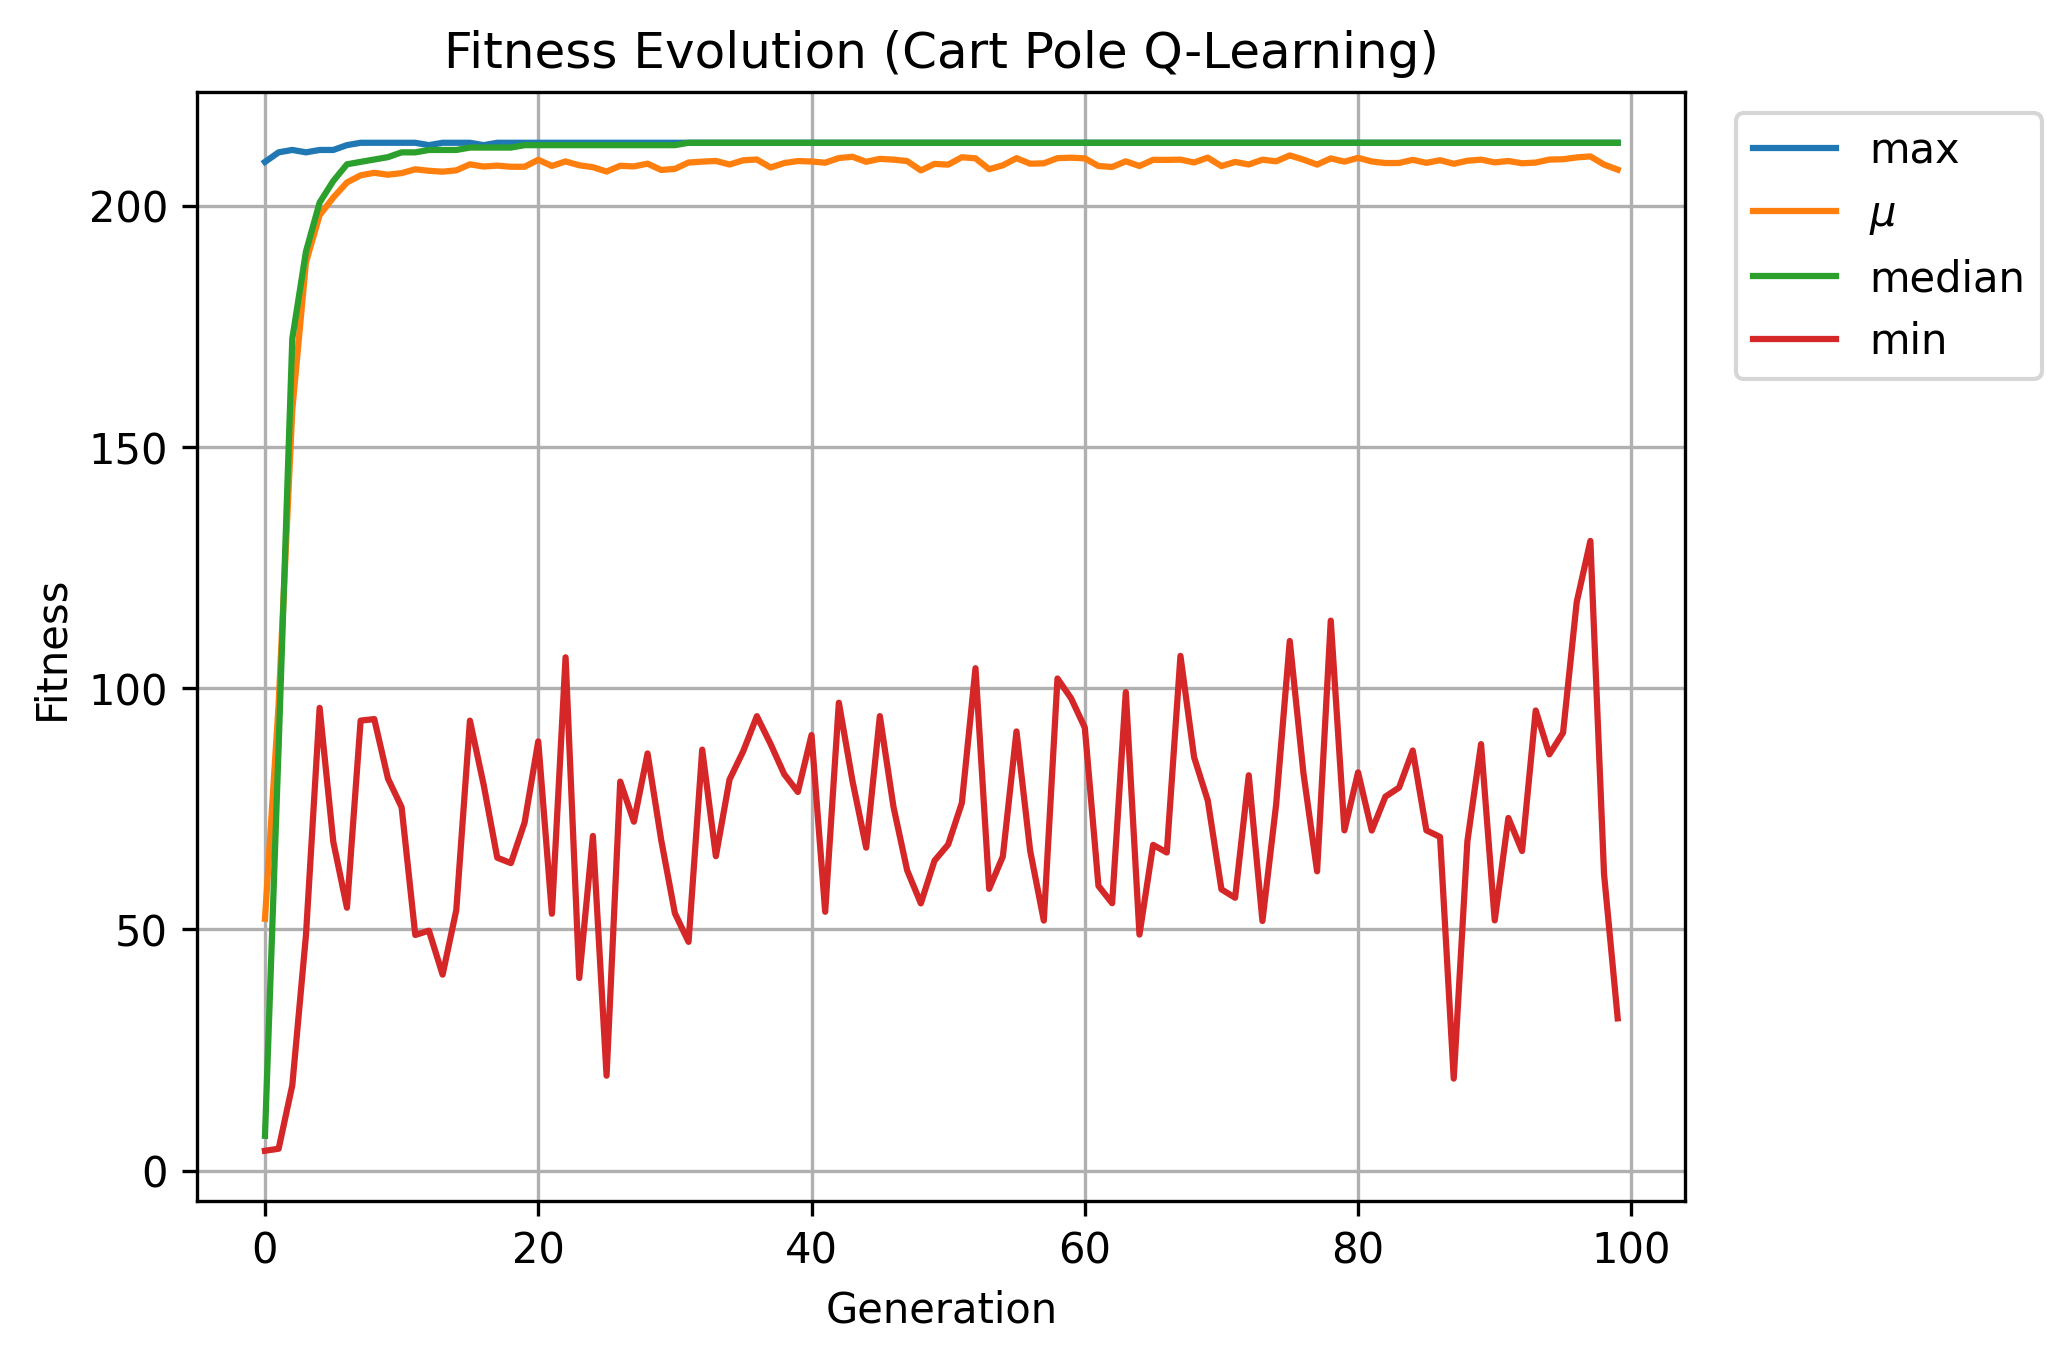
\includegraphics[width=\linewidth]{cart_pole_q.png}
		\caption{Linear Genetic Programming Reinforced with Q-Learning}
		\label{fig:cart-pole-q}
	\end{subfigure}
	\caption{Comparison of Cart Pole}
	\label{fig:cart-pole-comparison}
\end{figure}


\subsection{Mountain Car}

Figure \ref{fig:mountain-car-comparison} shows a comparison between the performance of individuals who were trained on the baseline LGP algorithm and the Q-Learning enhanced algorithm. The baseline program achieved a maximum of
-106, median of -110 and a mean of -122. The Q-Learning enhanced program achieved a maximum of -113, median of -115 and a mean of -132.

Both algorithms converged quickly to a score of -120 at around 10 generations.
There's a small positive increase seen once the baseline program converges, whereas there's a small negative decrease seen once the Q-Learning enhanced program converges.

Overall, both algorithms were able to solve the mountain-car-v0 environment in a reasonable amount of steps.

\begin{figure}[ht]
	\centering
	\begin{subfigure}{1.0\textwidth}
		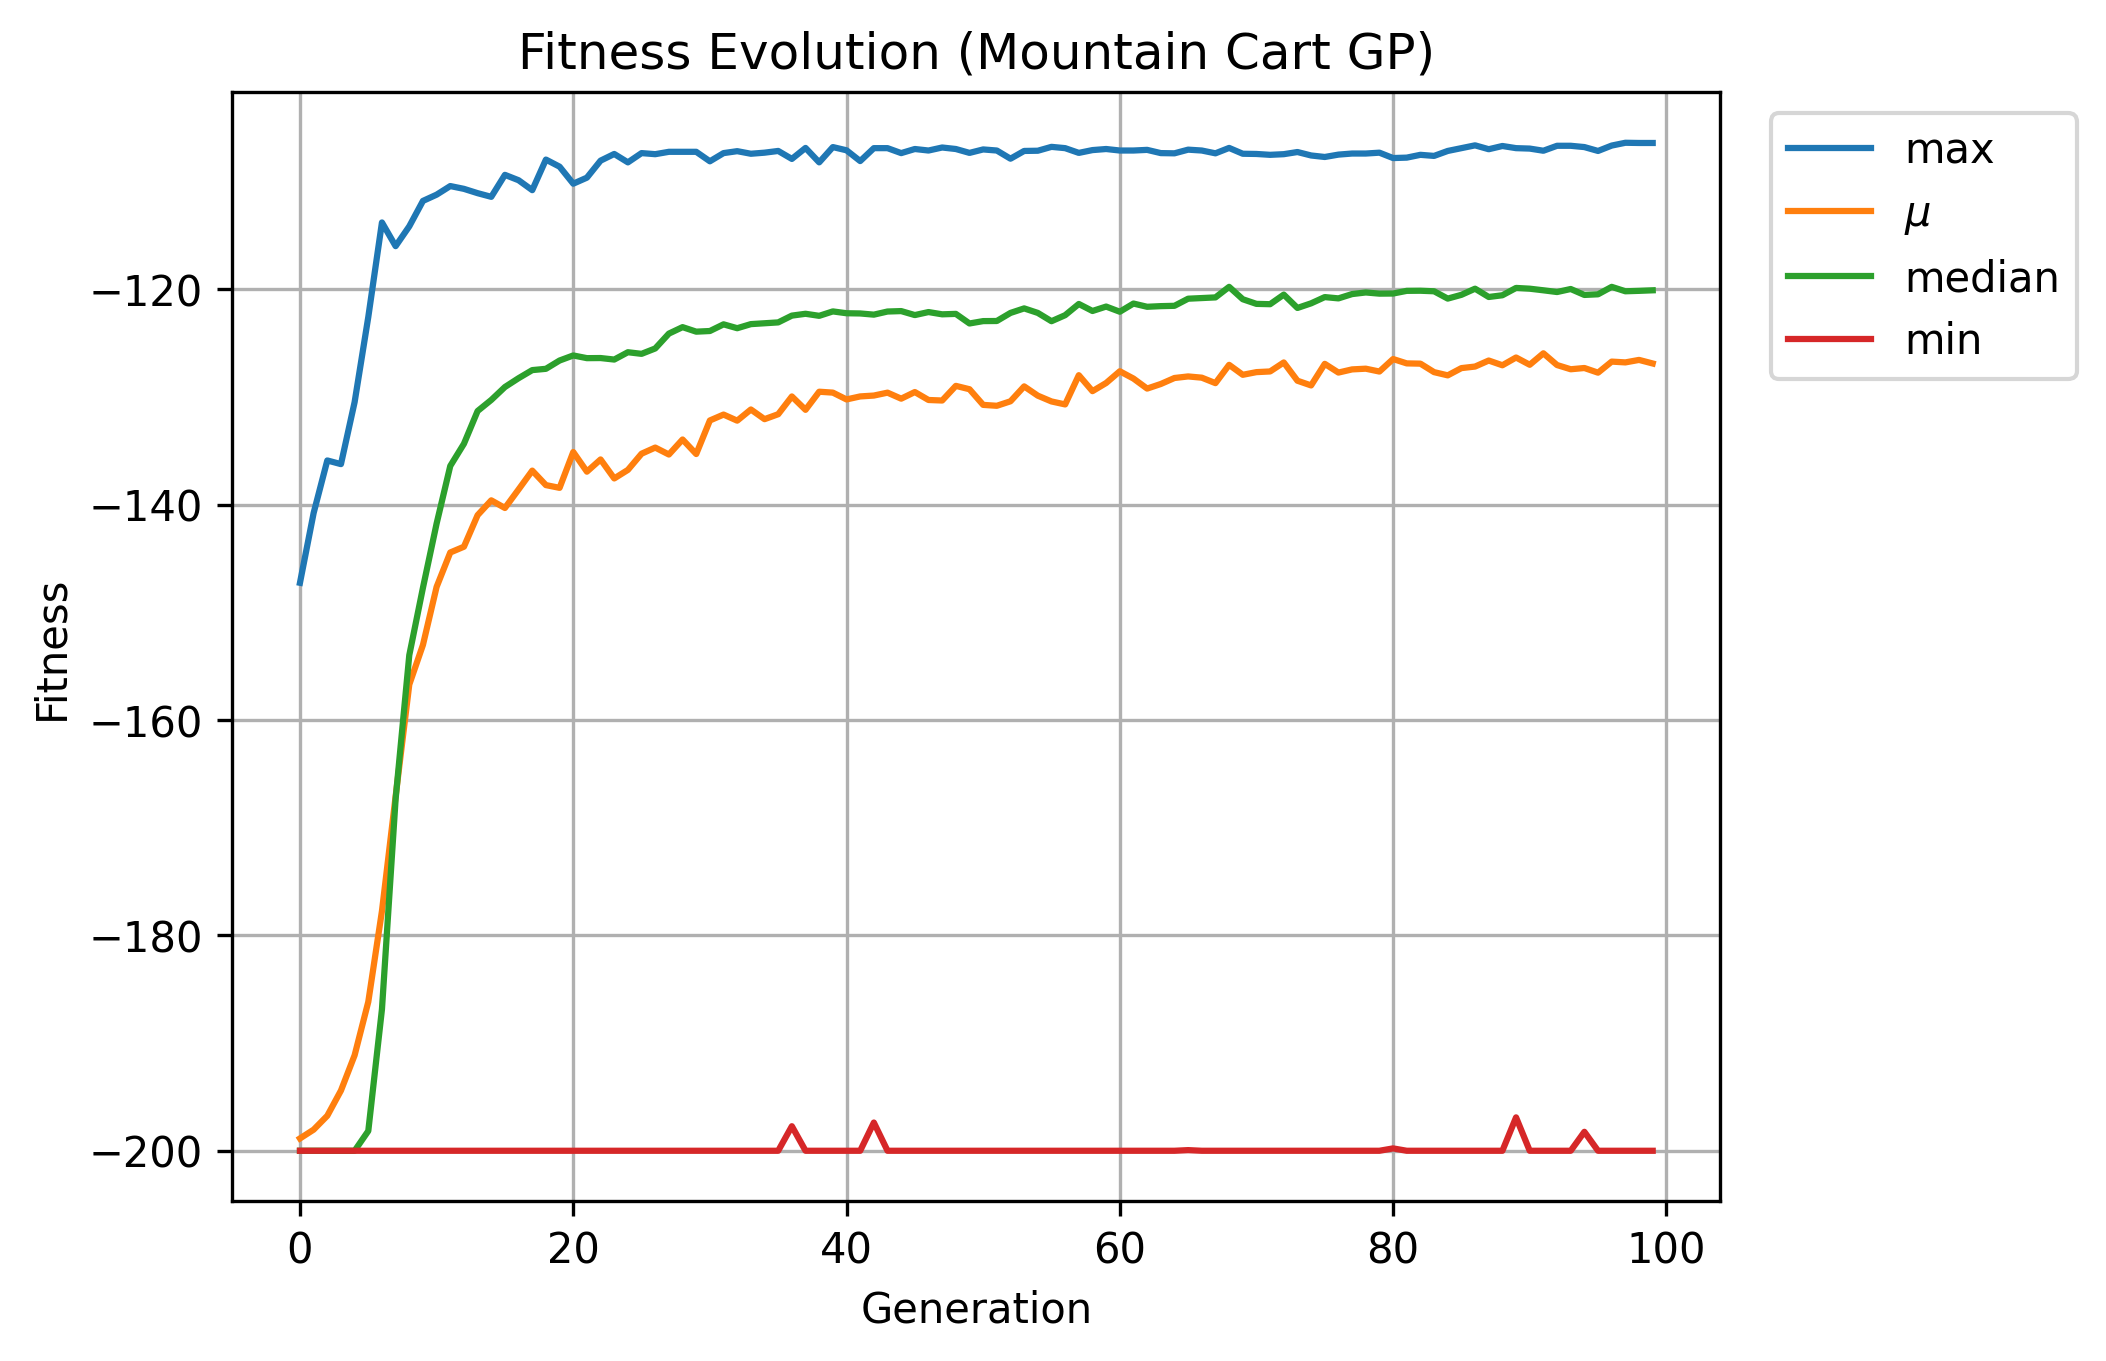
\includegraphics[width=\linewidth]{mountain_car_lgp.png}
		\caption{Baseline Linear Genetic Programming}
		\label{fig:mountain-car-lgp}
	\end{subfigure}
	\hfill
	\begin{subfigure}{1.0\textwidth}
		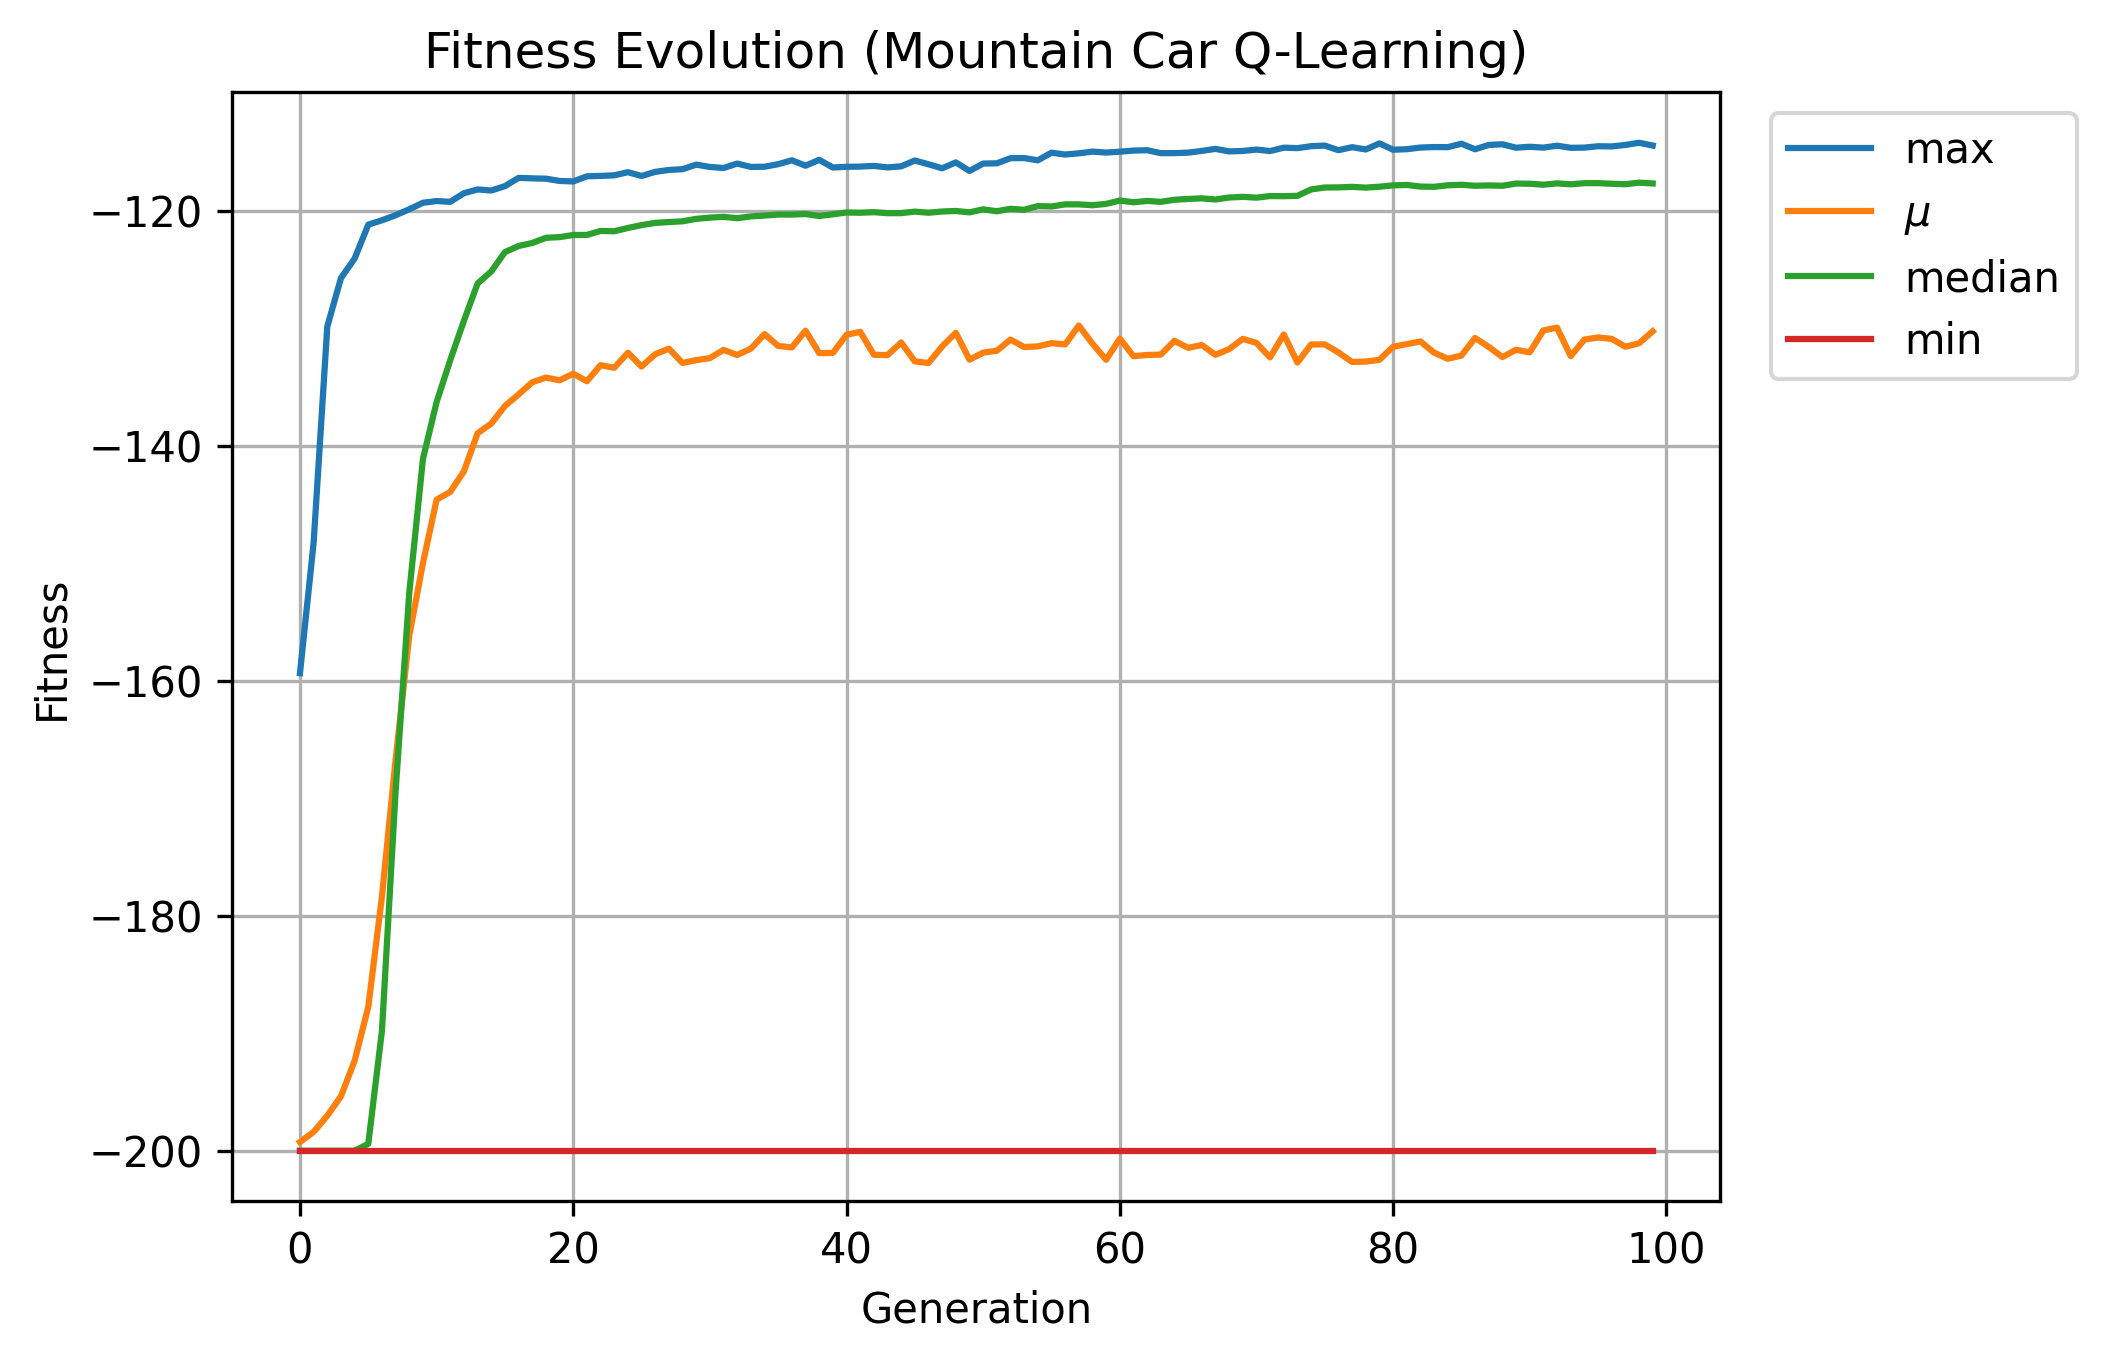
\includegraphics[width=\linewidth]{mountain_car_q.png}
		\caption{Linear Genetic Programming Reinforced with Q-Learning}
		\label{fig:mountain-car-q}
	\end{subfigure}
	\caption{Comparison of Mountain Car}
	\label{fig:mountain-car-comparison}
\end{figure}


\section{Discussion}
Q-learning and other reinforcement learning algorithms' performance can depend on various factors, such as the nature of the environment, state and action space, hyperparameters, and the exploration-exploitation balance.

In the case of the Mountain Car and Cart Pole environments, the differences in performance can be attributed to the following reasons:

\begin{enumerate}
	\item \textbf{State space}: The state space of Mountain Car is smaller and relatively simpler compared to Cart Pole. Mountain Car has two continuous variables (position and velocity), while Cart Pole has four (cart position, cart velocity, pole angle, and pole angular velocity). Q-learning can learn the simpler state space of the Mountain Car problem more effectively.

	\item \textbf{Exploration vs. Exploitation}: Q-learning uses an epsilon-greedy exploration strategy, which balances exploration (trying out new actions) and exploitation (choosing the best-known action). In the Mountain Car problem, exploration helps the algorithm find the optimal policy by trying various actions in different states. In the Cart Pole problem, the optimal policy might be harder to find, as even slight deviations in exploration can cause the pole to fall.

	\item \textbf{Reward structure}: The reward structure in Mountain Car is sparse, meaning the agent only gets a reward when it reaches the goal. In contrast, Cart Pole has a more dense reward structure, where the agent gets a reward for every time step it manages to keep the pole upright. Sparse rewards can sometimes make learning more difficult, but in this case, Q-learning seems to work well in the Mountain Car environment despite this challenge. In Cart Pole, the dense rewards can make it harder for Q-learning to differentiate between good and bad actions since the agent gets a reward for each time step it doesn't fail, which might lead to sub-optimal policies.

	\item \textbf{Hyperparameters}: The performance of Q-learning also depends on hyperparameters like learning rate, discount factor, and epsilon (exploration rate). These parameters might need different tuning for different environments. It is possible that the provided hyperparameters are better suited for the Mountain Car environment than the Cart Pole environment.
\end{enumerate}

When looking at the mean, median, and maximum scores achieved by the algorithms in both environments, we can observe that the baseline LGP program generally performs better than the LGP-Q program in the Cart Pole environment, with a higher maximum, median, and mean score. In contrast, the LGP-Q program converges faster in the Cart Pole environment, but plateaus at a lower score. In the Mountain Car environment, both algorithms converge quickly to a score of -120 and show similar performances. The small differences in maximum, median, and mean scores in the Mountain Car environment further highlight the factors discussed above, as they demonstrate how the nature of the environment, state space, and reward structure, as well as the choice of hyperparameters, can impact the performance of the algorithms.

\chapter{Conclusion}

Overall there seems to be some promise in using Q-learning.

\section{Future Work}
% Describe potential future steps and improvements for your research.

\bibliographystyle{plain}
\bibliography{thesis}

\end{document}
